\chapter{Evaluation}

The \acrshort{API} has been evaluated in three ways. First, a functional evaluation was performed, checking if the \acrshort{API} behaves as expected. Next, a latency evaluation was done, measuring if there are any noticeable slowdowns while using the \acrshort{API} compared to native code. Finally, a memory evaluation was constructed, measuring the impact on memory usage of running the code in \acrshort{Wasm} compared to native.

The code of all the benchmarks can be found in the \textit{USB\_WASI} \cite{usb_wasi_impl} repository.

\subsection{Test Setup}

This section will go briefly over the test setups used to perform the evaluation.
Table \ref{table:test_hardware} shows the hardware configurations of the devices used to do these tests. Table \ref{table:software_environment} shows the software environment in which the tests were performed.

\begin{table}[H]
\[
\begin{array}{|l|l|l|l|l|l|}
\hline
\textbf{Device} & \textbf{Name} & \textbf{SoC/Microcontroller} & \textbf{RAM} & \textbf{Storage} & \textbf{USB Version} \\
\hline
\text{Host} & \text{Apple Macbook Air (2020)} & \text{Apple M1 (8-core CPU, 7-core GPU)} & \text{8GB} & \text{256GB SSD} & \text{4.0} \\

\hline
\text{Guest} & \text{Arduino Micro} & \text{Atmel ATmega32U4} & \text{2,5KB} & \text{32KB Flash} & \text{2.1} \\

\hline
\text{Guest} & \text{Samsung T5 Portable SSD} & \text{Unknown} & \text{Unknown} & \text{500GB SSD} & \text{3.1 Gen 2} \\
\hline
\text{Guest} & \text{Google Stadia Game Controller} & \text{NXP MIMXRT1061} & \text{1024KB} & \text{16MB} & \text{2.0} \\
\hline
\end{array}
\]
\caption{The hardware used for testing the performance of the API.}
\label{table:test_hardware}
\end{table}

\begin{table}[h]
\centering
\begin{tabular}{|l|l|}
\hline
\textbf{Operating System} & macOS 14.5 \\ \hline
\textbf{Wasm Runtime} & Wasmtime 20.0.2 \\ \hline
\textbf{USB Library} & libusb 1.0.27, Rusb 0.9.4 \\ \hline
\textbf{Rust Version} & rustc 1.78.0 \\ \hline
\end{tabular}
\caption{Software Environment.}
\label{table:software_environment}
\end{table}

\begin{figure}[H]
  \centering
  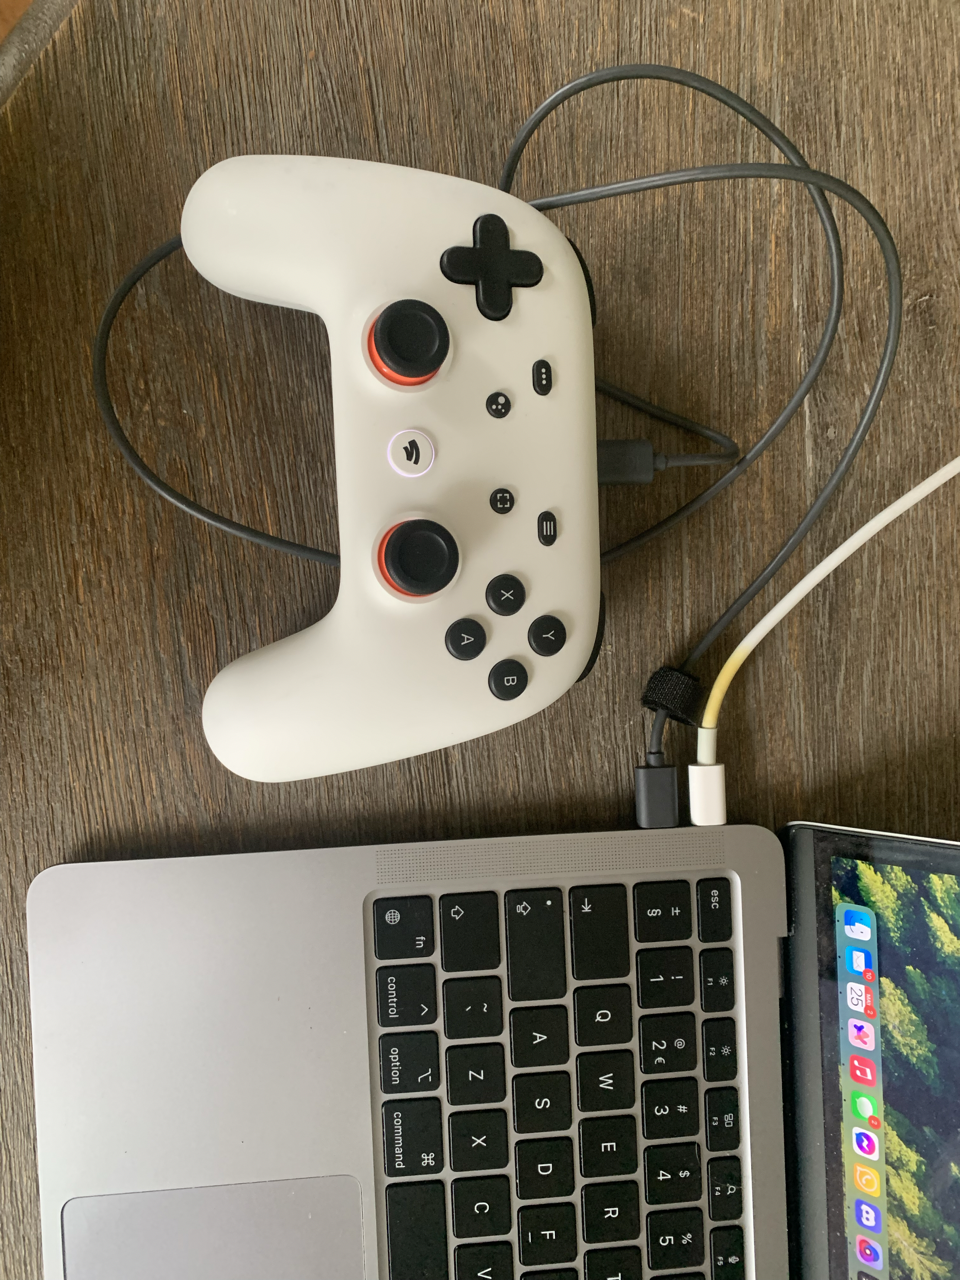
\includegraphics[width=0.5\textwidth, angle=90]{images/stadia_setup.png}
  \caption{Setup for testing with the Google Stadia controller. The controller is directly connected to the host device with an USB 2.0 C to C cable.}
  \label{fig:stadia_setup}
\end{figure}

\begin{figure}[H]
  \centering
  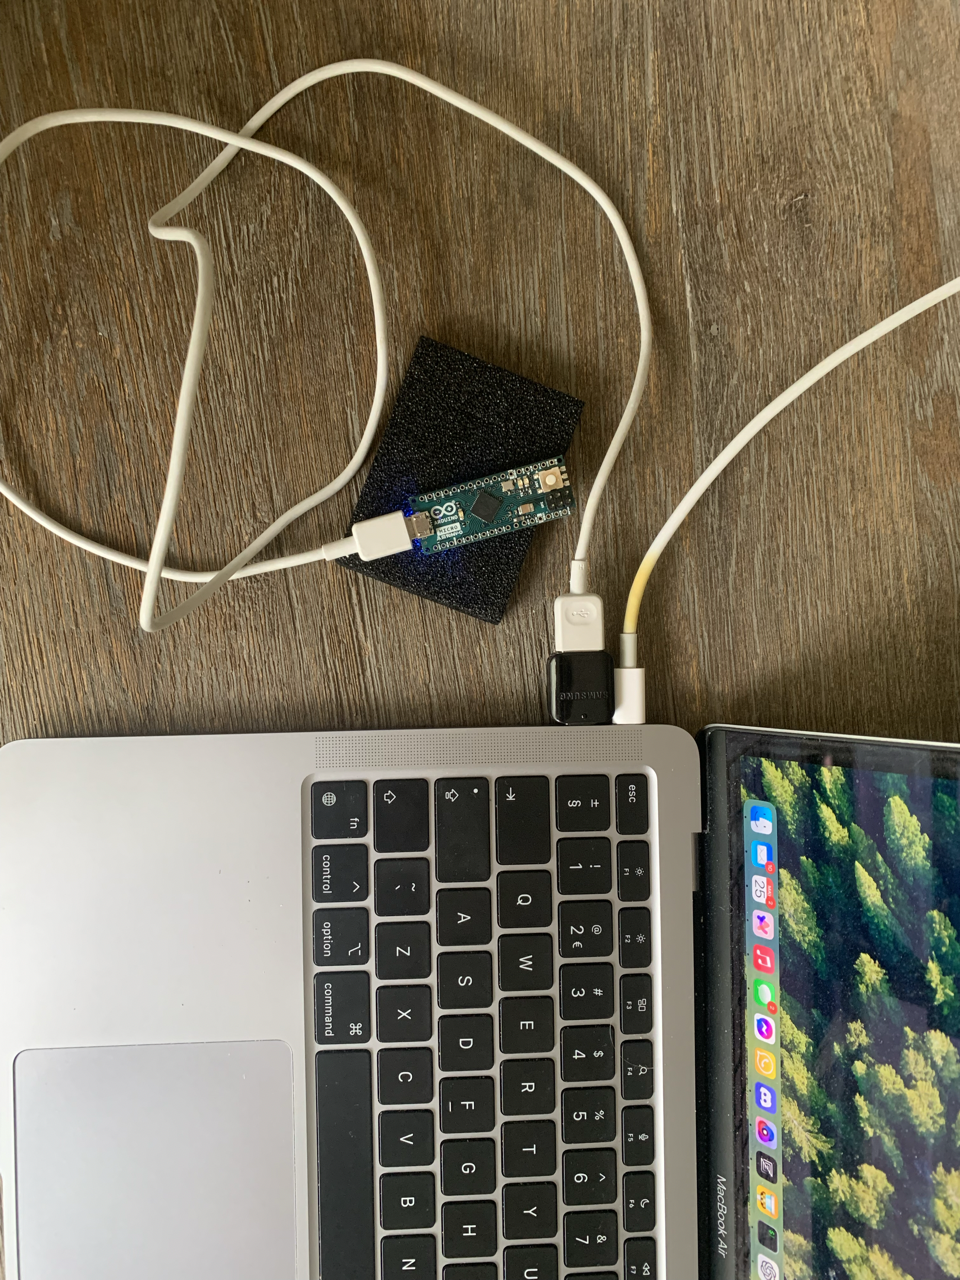
\includegraphics[width=0.5\textwidth, angle=90]{images/arduino_setup.png}
  \caption{Setup for testing with the Arduino board. The Arduino is connected via a USB 3.0 A to C adapter, and a USB 2.0 B to A cable.}
  \label{fig:arduino_setup}
\end{figure}


\begin{figure}[H]
  \centering
  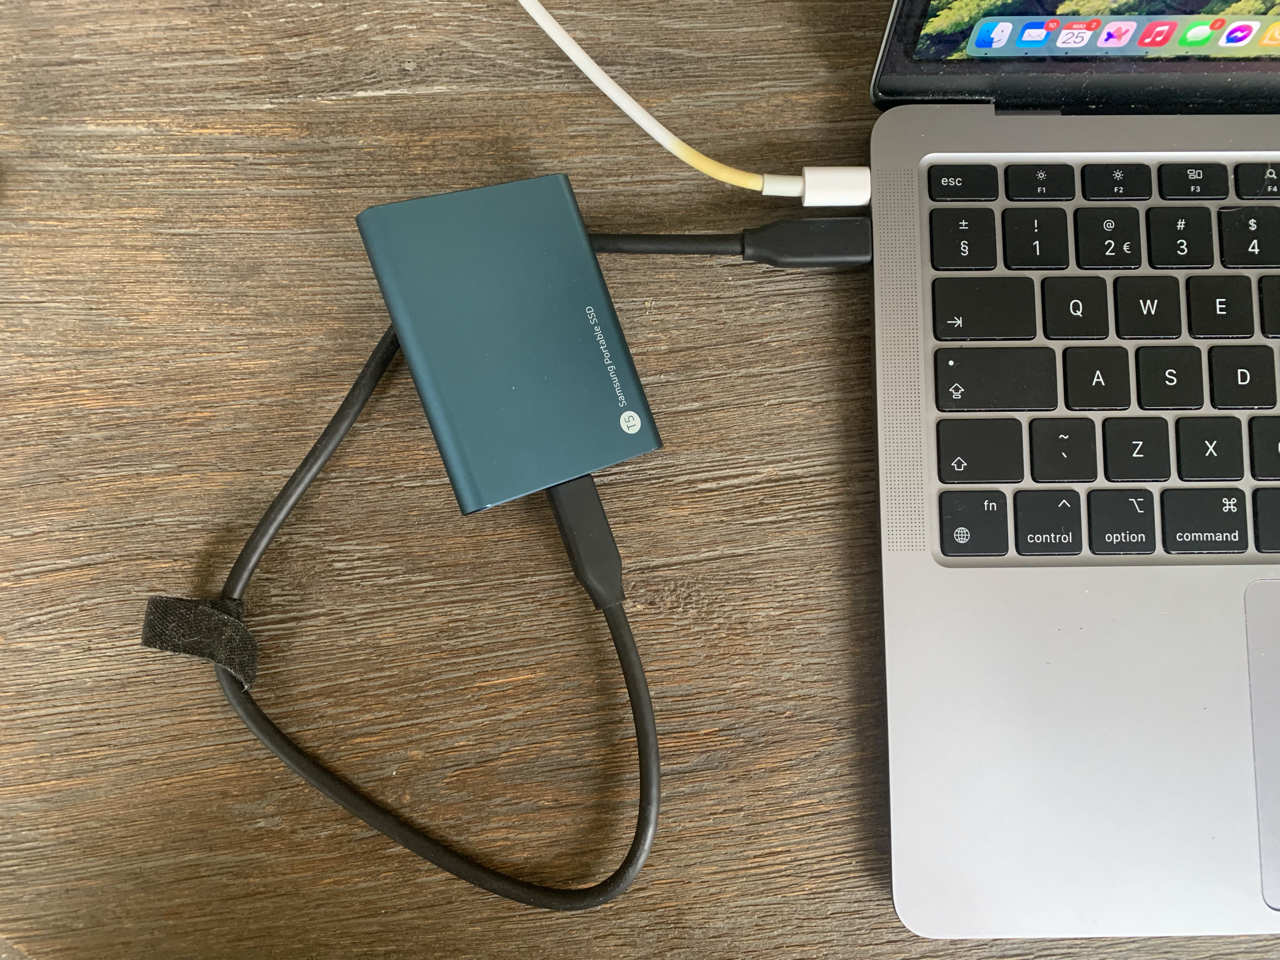
\includegraphics[width=0.7\textwidth]{images/t5_setup.png}
  \caption{Setup for testing the Samsung T5 SSD. The SSD is directly connected to the host device with a USB 3.1 Gen 1 (5Gbps) C to C cable.}
  \label{fig:samsung_setup}
\end{figure}




\section{Functional Evaluation}
\label{section:functional_evaluation}
When developing the API, it is useful to already have guest code utilizing the API to quickly iterate. The following proof of concept is one of the guest programs created to test the API. It touches on all parts of the API: Getting device connection and disconnection events, reading descriptors from a device, opening a device handle, reading data from the device and writing data to the device. As it is a functional evaluation, it does not test the performance of the API.

The general idea of the program is to control a game controller. The program is started and observes the connected devices. Once a controller is connected that is recognized by the program, the program will connect to the controller. The state of all the controls of the device will be read, and input updates will be print out. To test sending data over the USB interface, the program will send commands to the controller to activate the rumble motors \footnote{Rumble motors are used to vibrate the controller}. If the program receives a disconnection event, it will stop reading data and become idle again, waiting for new connections.

\subsubsection{Test Methodology}
The code will call the event-related API to start watching for USB devices. It will get events when devices are connected or disconnected. As WASI does not support asynchronous code yet \cite{wasi_roadmap}, a form of polling is used to get device connection events. The guest code uses a single-threaded asynchronous runtime, which will often yield to get new device connection events. This way, a multi-threaded real app can be simulated.

\begin{enumerate}
\item Each time a device connection event happens, the device product and vendor ID are checked to see if they match the predefined controller product and vendor ID. A Google Stadia controller is used to test this code, so the IDs of this controller type are used.

\item Make a connection and open a device handle if the device IDs match.

\item Select the correct configuration and interface. Input devices, like controllers or mice, send their data over the Interrupt transfer type, because the data sent is small and time-sensitive. Knowing this information, the interfaces can be requested and filtered to select the correct interface. macOS is used to run this example which offers default drivers for controllers, so elevated privileges are needed to detach the kernel drivers. Otherwise, the program cannot claim the interrupt interface.

\item Read the controller state from the interrupt interface, such as which buttons are pressed, what the position of the joysticks is, etc. An array of bytes is received, and by observing changes to this array when pressing a button, the byte layout can be decoded.

\item Print out the controller state. A sample output is showed in Code snippet \ref{code:wasi_controller_sample_output}.

\item Make the controller vibrate. This happens when the program state reports that one of the shoulder buttons has registered pressure. The state of the shoulder buttons is mapped to intensity of the rumble motors. This data is sent over the interrupt interface. When the controller receives the data it starts vibrating.

\item When a device disconnection event with matching IDs happens, the program will stop reading the controller state, close the device handle, and wait for a new connection.


\end{enumerate}

% Each time a device connection event happens, the device product and vendor ID are checked to see if they match the predefined controller product and vendor ID. A Google Stadia controller is used to test this code, so the IDs of this controller type are used. If the IDs match, a connection is made to the device by opening a device handle. When a device disconnection event with matching IDs happens, the program will stop reading the controller state, and wait for a new connection.
% 
% Next, the program will try reading the controller state. This way, it knows about the positions of buttons, joysticks, triggers, etc. In order to do this, the correct interface and endpoint must be chosen. Input devices, like controllers or mice, send their data over the Interrupt transfer type, because the data sent is small and time-sensitive. Knowing this information, the interfaces can be requested and filtered to select the correct interface. In order to send information over the interface, it must first be claimed by the program. Some operating systems will attach to the interfaces by default. The host code of the API will automatically disconnect kernel attachments when claiming an interface. However, different operating systems can have different behavior in this part. For example, macOS, where the example program was ran on, does not allow detaching kernel interfaces by default for certain device classes, such as controllers. This is problematic, as we cannot interact in any way with the device this way. Elevated privileges (\texttt{sudo}) were required to get the program working. While being annoying, this was also a useful discovery, as this issue can be added to the proposal, so the standard can adjust to this.
% 
% Once the interface is claimed, device state can be requested by reading the interrupt state with the correct endpoint address. An array of bytes will be received, and by observing what changes when pressing a button, the byte layout can be decoded. A sample controller state output is showed in Code snippet \ref{code:wasi_controller_sample_output}.

\begin{code}
\begin{verbatim}

dpad: ,
buttons: assistant_button|l2_button|r2_button,
left stick: x: 128 y: 128,
right stick: x: 128 y: 128,
l2: 255,
r2: 172
\end{verbatim}
\caption{Output after reading controller state.}
\label{code:wasi_controller_sample_output}
\end{code}

\subsubsection{Results}
This program has been tested with a Google Stadia controller. When pressing one or multiple buttons, the correct state is printed out. When pressing one or both of the shoulder buttons, the controller starts to vibrate.



\section{Latency Evaluation}

One of the advantages of \acrshort{Wasm} should be that it offers near-native speed. Therefore, it is interesting to test if running a program in Wasm brings any performance overhead compared to a native program. For an USB API, this can best be tested by measuring the latency when sending or receiving data. It can be problematic if the overhead is large, as data exchange through USB happens by receiving or sending data in small chunks. Each of these chunks has to pass through the Wasm bridge and has its own overhead.

\subsection{Receiving data from Arduino}

\subsubsection{Test Methodology}
A program has been written with LibUSB (Native) and WASI USB (Wasm). Each program will do the following steps:

\begin{enumerate}
\item Enumerate the USB devices.
\item Find the Arduino board, based on its product and vendor id.
\item Open the device and claim the Bulk interface.
\item Send the \acrfull{DTR} signal to the Arduino. This signal is sent to the Arduino to acknowledge that the host device is ready to receive data. Once the Arduino has received this signal, its setup phase is completed and it will start sending data.
\item \textit{Warm up } the interface by throwing away the first batch of readings. By doing this, initial latency is removed from the measurements.
\item Read data from the Bulk interface, while measuring how long this operation takes. The arduino sends data in batches in 64 bytes, and the program will read them a million times. The program will throw away the read results, so only the transfer of the data is measured. In total, 64MB is received by the host.
\item Write durations to file.
\end{enumerate}

\subsubsection{Results}
Figure \ref{fig:arduino_reading_latency_boxplot} shows a boxplot of the latencies of both programs. After a million measurements for each program, the median duration is exactly the same, 377μs. The average of the native program is marginally lower, being 0.2\% faster than the \acrshort{WASI} program. The whiskers and IQR of the \acrshort{WASI} program are slightly smaller, meaning a more consistent result. However, the differences in results are too small to conclude any noticeable overhead.

\begin{figure}[H]
  \centering
  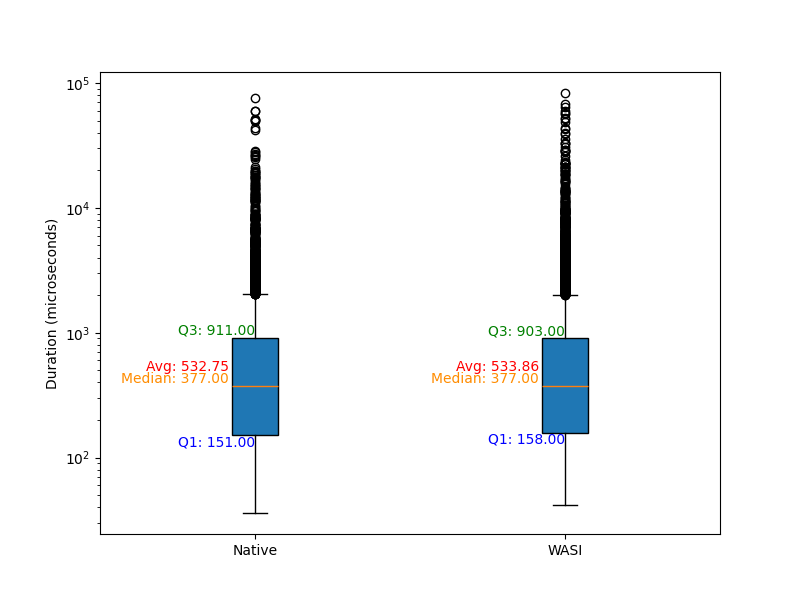
\includegraphics[width=1\textwidth]{images/arduino_latency_boxplot.png}
  \caption{Latency of reading data from Arduino using read-bulk.}
  \label{fig:arduino_reading_latency_boxplot}
\end{figure}


Figure \ref{fig:arduino_reading_latency_boxplot} also contains outliers, marked by the black circles. Some of the outliers are very large. Therefore, the results are shown on a logarithmic scale. These outliers are likely caused by transmission errors when receiving data from the Arduino. The \textit{Bulk} interface is used, providing data integrity but no timing guarantees. Consequently, data loss will be prevented, but will introduce high latencies as observed here. Table \ref{table:latency_comparison} shows more information about the outliers. As the percentage of outliers is very small and occur in equal quantities in both cases, they have been excluded from further figures to improve the clarity of the graphs.

\begin{table}[h]
\centering
\begin{tabular}{|l|c|c|}
\hline
 & \textbf{Native} & \textbf{WASI} \\ \hline
\textbf{Largest Outlier (μs)} & 75618 & 83052 \\ \hline
\textbf{Amount of Outliers (\textgreater 2000 μs)} & 747 & 1058 \\ \hline
\textbf{Percentage of Total} & 0.07\% & 0.10\% \\ \hline
\end{tabular}
\caption{Comparison of Latency Outliers between Native and WASI.}
\label{table:latency_comparison}
\end{table}



Figure \ref{fig:arduino_reading_latency} shows a \acrfull{KDE} for the measurements of the native and \acrshort{WASI} implementation.
Both graphs will show peaks around the 150μs and 910μs marks. This is an interesting result, as one would expect one uniform distribution instead of two. The first peak is trivial to explain: the Arduino is an USB 2.0 device, also known as a High-speed USB device. A High-speed USB device will send frames at a fixed interval of 125μs. Therefore, we will receive new data approx. every 125μs. An extra 25μs are introduced because of processing delays. 

The second peak is more nuanced. Table \ref{table:arduino_output} shows a snippet of the measured latencies. For both Native and WASI code, the latencies will oscillate between both peaks. Based on these results, this peak is likely caused by the small buffer size in the Arduino. The buffer is 64 bytes large, which is the same size as one packet. When the buffer is full, the program halts until the buffer has space again. On the host this is perceived as an extra delay when receiving the data.

\begin{figure}[H]
  \centering
  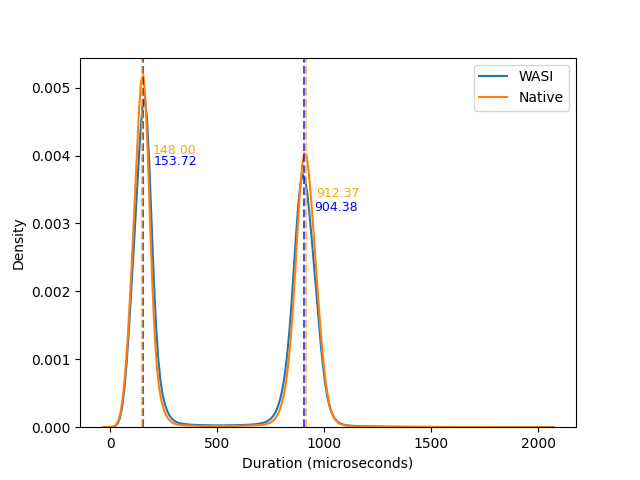
\includegraphics[width=1\textwidth]{images/reading_data_latency.png}
  \caption{Latency of reading data from Arduino using read-bulk.}
  \label{fig:arduino_reading_latency}
\end{figure}

\begin{table}[h!]
\centering
\begin{tabular}{|l|l|}
\hline
\textbf{Native (μs)} & \textbf{WASI (μs)} \\
\hline
801 & 918 \\
\hline
150 & 163 \\
\hline
885 & 931 \\
\hline
132 & 241 \\
\hline
903 & 799 \\
\hline
110 & 197 \\
\hline
938 & 820 \\
\hline
104 & 77 \\
\hline
962 & 1003 \\
\hline
108 & 97 \\
\hline
\end{tabular}
\caption{Snippet of measured latencies. The latencies oscillate between a long latency and a short latency.}
\label{table:arduino_output}
\end{table}

Based on the results, we can conclude that there are no measurable differences between the native and \acrshort{WASI} program. However, this is mainly caused by the delay of the USB protocol. This delay vastly outweighs the delays caused by overhead of the Wasm runtime, making the Wasm overhead negligible.

However, it is possible that the delay of the USB protocol is smaller on devices more powerful than an Arduino or with a more modern USB version. With these configurations, it can be possible a small overhead for Wasm becomes visible.

\subsection{Reading files from Mass Storage device}
\label{section:mass_storage_latency}

In order to confirm that WASI does not add noticeable latency, another benchmark is performed, which reads the contents of an USB mass storage device. The advantage of this benchmark compared to the Arduino benchmark is that it better represents real-world usage, instead of being a synthetic benchmark.

\subsubsection{Test Methodology}
A program has been written which enumerates the file tree of a USB device and reads the contents of each file in the file tree. A Samsung T5 External SSD is used to perform these tests. The device is connected with a cable that supports a transfer speed up to 5Gb/s and is formatted with the \acrshort{MBR} partition map and the \acrshort{exFAT} file system. There are 10 files stored on the device, most of which are a few KBs in size. One file has a size of 679MB. In total, 680MB is stored on the device.

The program contains a working but incomplete implementation for the \acrshort{USB} mass storage Bulk-Only transport specification. Further information about the specification and implementation details can be found in the specification documents \cite{usb_specification_boot} \cite{usb_specification_bulk}. The code exposes an interface where one can \textit{seek} to a specific address and \textit{read} the contents from there up until a specified length.

\paragraph{\acrshort{USB} \acrshort{API} Usage}
As the name of the specification suggests, communication with the device happens on the interfaces with the \textit{Bulk} transfer type. Some exceptions, such as the \texttt{reset} command, will use the \textit{Control} transfer type on interface zero.

\paragraph{Reading drive contents}
The \acrshort{USB} mass storage implementation acts as the base layer to communicate with the device. However, further abstraction is required. USB mass storage devices can still differ in numerous ways:

\begin{itemize}
\item Partition Map: A disk is usually split up in multiple partitions. A partition map contains information about those partitions. It is located in the first sector (sector 0) of the device. Popular partition maps are the \acrfull{MBR} and the \acrfull{GPT}. The test device has a \acrfull{MBR} partition map. The Rust package \textit{mbrman} \cite{mbrman} is used to read the \acrshort{MBR} and obtain the start and end addresses of the partition which contains the file system.

\item File System: The file system organizes files and their metadata in a defined format. There exist a lot of file systems, but the most popular for mass storage devices are \acrfull{FAT32}, \acrfull{exFAT} and \acrfull{NTFS}. The test device uses the \acrshort{exFAT} file system. The test program uses the \textit{exfat} \cite{exfat_package} Rust package to interpret the \acrshort{exFAT} partition.
\end{itemize}

Both \textit{mbrman} and \textit{exfat} use the mass storage implementation to read data at addresses. Code snippet \ref{code:implementation_mass_storage} shows how the mass storage implementation is used to read the files.

\begin{code}
\begin{minted}[breaklines, tabsize=4]{rust}

fn main() {
    // Open the mass storage device.
    let mut device = MassStorageDevice::new()?;
    let block_length = device.capacity.block_length;

    // Read the MBR to get information about the device partitions.
    let mbr = mbrman::MBR::read_from(device, block_length)?;

    // Select the first used partition.
    let data_partition = mbr.iter().find(|p| p.1.is_used())
        .ok_or(anyhow!("No used partition found"))?.1;

    // Apply a slice to the device stream, so only the selected partition is considered when reading.
    let slice_start = ...
    let slice_end = ...
    let slice = IoSlice::new(device, slice_start, slice_end)?;

    // Apply buffering to the stream to increase performance.
    let buffered_stream = BufReader::new(slice);
    
    // Open the exFAT file system.
    let filetree = ExFat::open(buffered_stream)?;

    // Recursively read the device tree.
    for item in filetree {
        read_item(item)?;
    }
}
\end{minted}
\caption{Code to read files and directories from the mass storage device.}
\label{code:implementation_mass_storage}
\end{code}

With a working implementation to read out the file tree, a benchmark can be performed. The benchmark enumerates the file tree and reads out the contents of each file, and reports each file size and name. The duration of this operation is logged. This is repeated 1000 times, so the file tree will be read out 1000 times. This is done for the program running in Wasmtime using the \acrshort{USB} \acrshort{API} and a native program using Rusb \cite{rusb}.

\subsubsection{Results}

Figure \ref{fig:mass_storage_latency_naive} shows a boxplot with the results of reading the file tree and file contents of the device. With a lower average and median, the \acrshort{WASI} program seems to outperform the native program. The average execution time of the native program is 12\% slower than the \acrshort{WASI} program, the median execution time is 18\% slower. This is odd, as one would expect the native version to be faster.

However, there is an explanation for this behaviour. The program will read out the entire contents of the disk, which is in total around 3GB. Each file will be loaded into memory and immediately discarded. The disk contains a few files with a size of over 500MB. Loading these files into memory becomes expensive due to the amount of \texttt{malloc}s that need to happen. Profiling the code shows more insights.

The code is compiled in debug mode so debug symbols are added to both programs, so we can interpret the system calls easier. This will lead to a significantly slower running program, especially for the \acrshort{WASI} program. This is not a problem as the profiling is only used to measure memory usage and not speed. The sample size is also lowered to 10 samples instead of 1000.

Figure \ref{fig:malloc_instruments} shows the total time spent on \texttt{malloc} for the native program. 25\% of the execution time was spent on allocating memory, which is a significant amount. Figure \ref{fig:malloc_wasi_instruments} shows that the \acrshort{WASI} program only spends 0.6\% of its execution time on \texttt{malloc} and therefore does not have this issue. This happens because of the way a \texttt{Store} works in Wasmtime: \say{A Store is intended to be a short-lived object in a program. No form of GC is implemented at this time so once an instance is created within a Store it will not be deallocated until the Store itself is dropped.} \cite{wasmtime_store}. Because no memory is freed, the already-allocated memory can be reused, avoiding extra \texttt{malloc} and \texttt{free} calls. A Wasmtime \texttt{Store} therefore can act as a memory pool, which can be significantly faster than using \texttt{malloc} \cite{memory_pool_wikipedia}.


\begin{figure}[H]
  \centering
  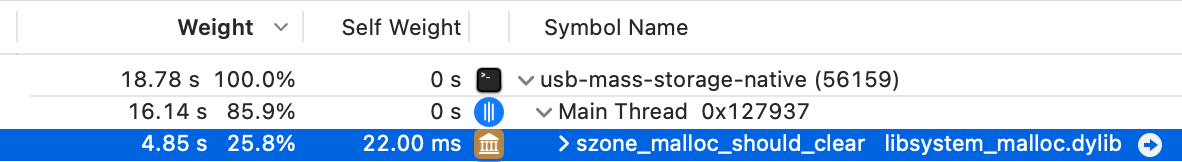
\includegraphics[width=1\textwidth]{images/malloc_screenshot.png}
  \caption{Approx. 25\% of the native program execution time is spent on \texttt{malloc}.}
  \label{fig:malloc_instruments}
\end{figure}

\begin{figure}[H]
  \centering
  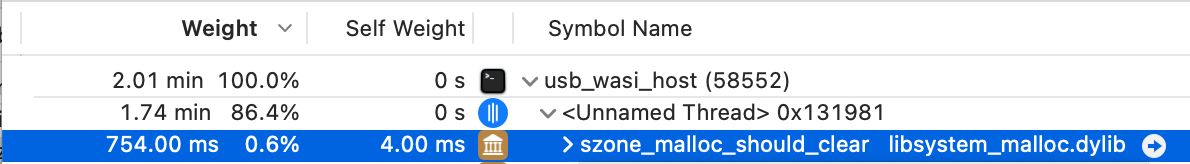
\includegraphics[width=1\textwidth]{images/malloc_wasi_screenshot.png}
  \caption{Approx. 0.6\% of the \acrshort{WASI} program execution time is spent on \texttt{malloc}.}
  \label{fig:malloc_wasi_instruments}
\end{figure}

\begin{figure}[H]
  \centering
  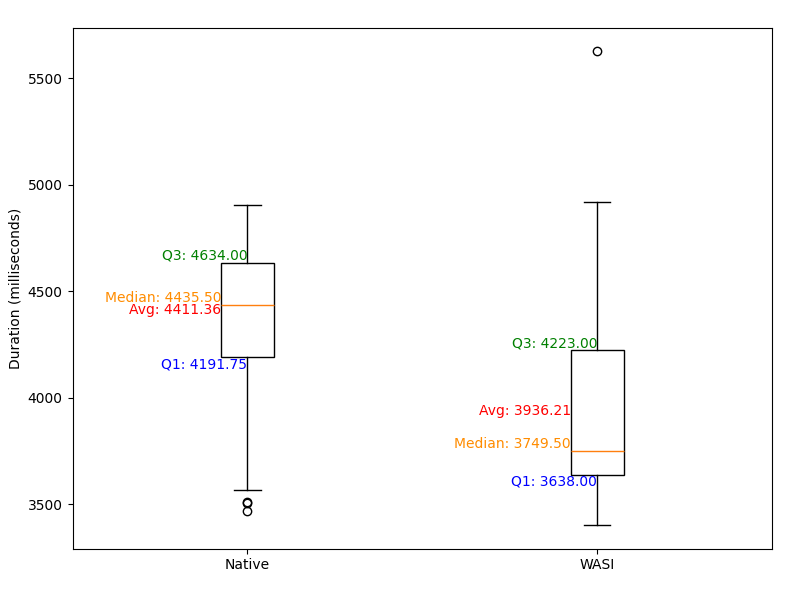
\includegraphics[width=1\textwidth]{images/mass_storage_1000_runs_naive.png}
  \caption{Latency of reading the file tree and contents. The \acrshort{WASI} results incorrectly report a better result due to differences in memory allocation between both programs. On average, the native program is 12\% slower.}
  \label{fig:mass_storage_latency_naive}
\end{figure}



\subsubsection{Improving results}

To make a better measurement at the latency of the \acrshort{USB} \acrshort{API}, the test has been modified. Instead of the test running multiple times in the guest code, the guest component runs multiple times. Each time, a new \texttt{Store} will be created. This will let the memory allocation behave similar to the native program.

Figure \ref{fig:mass_storage_latency_optimized} shows a boxplot with the new measurements. The measurements of the native program are the same as in Figure \ref{fig:mass_storage_latency_naive}. The average \acrshort{WASI} program execution time is 4.2\% slower than the average native program, and the median 4.3\% slower. The \acrshort{WASI} program also has more outliers, indicating that the performance of the \acrshort{WASI} program may be less consistent.

\subsubsection{Conclusion}
Based on these results, we can conclude that running the code using the \acrshort{WASI} \acrshort{USB} \acrshort{API} introduces a small amount of overhead. Caution must be exercised when benchmarking memory-intensive \acrshort{Wasm} programs to obtain accurate results.

\begin{figure}[H]
  \centering
  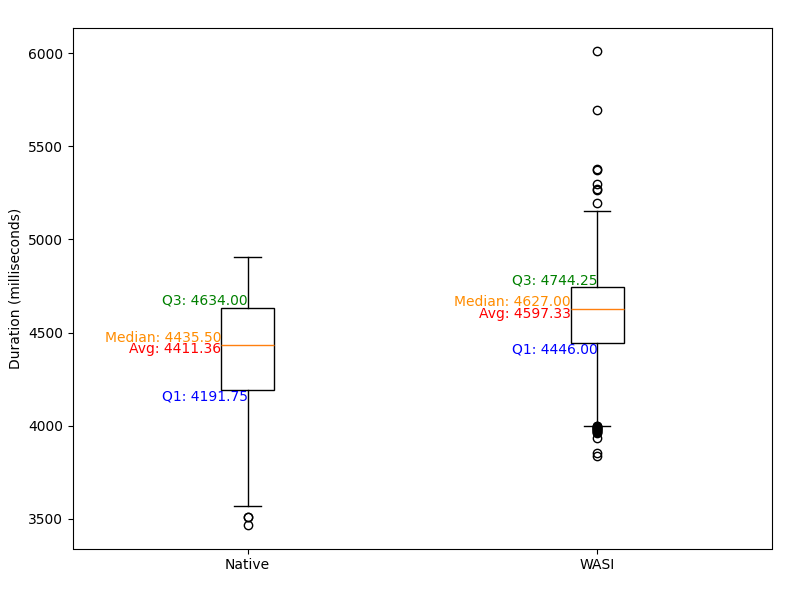
\includegraphics[width=1\textwidth]{images/mass_storage_1000_runs_optimized.png}
  \caption{Latency of reading the file tree and contents after changing the benchmark method. Both programs now use a similar memory allocation method leading to more accurate results. On average, the \acrshort{WASI} \acrshort{USB} implementation is approx. 4.2\% slower.}
  \label{fig:mass_storage_latency_optimized}
\end{figure}

\section{Memory Usage Evaluation}
In contrast to standard \acrshort{Wasm} modules, \acrshort{WASI} components have separate memory spaces. As a result, one component cannot read or write the memory of another component \cite{memory_model}. This improves the security of the Component Model and the interoperability between components, but can also add additional memory usage due to the need of copying memory. Therefore, it is interesting to see how much impact \acrshort{WASI} has on the memory usage of a typical program.

\subsection{Reading files from mass storage device}
\label{section:reading_files_memory}
The same test methodology as Section \ref{section:mass_storage_latency} will be used to benchmark memory usage. Section \ref{section:mass_storage_latency} already discussed a performance issue caused by memory allocation. As this section is about the \textit{amount} of memory used, and not about the \textit{performance} of utilizing it, this problem won't be further discussed here.

\subsubsection{Test Methodology}
\label{section:reading_files_memory_test_setup}
Some changes are made to the test methodology described in \ref{section:mass_storage_latency}. Instead of logging the duration of reading the file tree, the amount of memory will be logged. Also, instead of running the benchmark 1000 times, it is now run once.

The method to measure the memory will differ slightly in both implementations. Using a profiler to measure the memory has given incorrect results when benchmarking the \acrshort{WASI} implementation. Therefore, no profiler is used for this benchmark. Instead, the memory size is checked numerous times during the execution of the program. This is done getting the \textit{real} memory size of the program every millisecond. For the \acrshort{WASI} program this is done in Wasmtime. A baseline memory usage is also measured for the \acrshort{WASI} program which gets loaded but does not do anything.

The program will also sleep three seconds before and after opening and closing the device, so the memory usage evolution can be better seen.

\subsubsection{Results} 

Figure \ref{fig:mass_storage_memory_comparison} shows the differences in memory usage for both programs. As both programs consume a lot of memory, the initial Wasmtime memory usage is neglected, as it does not have a large influence on the results. The influence of initial Wasmtime memory is discussed in Section \ref{section:travering_file_tree_memory}.

After the initial three seconds of waiting time, both programs start traversing the file tree and reading the contents. It is clear that the \acrshort{WASI} program uses more memory and with more spikes. As memory is not shared, values are copied over from host to guest, increasing the memory usage. At its peak, it will use 1239MB, while the native program uses 718MB. This is 72.5\% more. This peak happens when reading in the largest file of 679MB. As the disk is mostly empty, data is stored contiguously on the disk. This improves reading performance and ensures a steady flow of data at the receiver's end. This is clearly visible in the graph for the native program, as its memory usage follows a linear function. The \acrshort{WASI} implementation contains more spikes. These spikes are likely caused by the copying of values, which rapidly allocates and deallocates memory.

After the contents have been read, memory usage will quickly drop for both programs. However, memory usage for the \acrshort{WASI} program will decrease slower than the native program. This mainly happens because of the memory-pool-like behavior of the \texttt{Store} \cite{wasmtime_store}, which will not deallocate memory. Memory used outside the \texttt{Store} will still get deallocated, which is why there is a memory decrease. Once the program ends the memory will get freed further.

\begin{figure}[H]
  \centering
  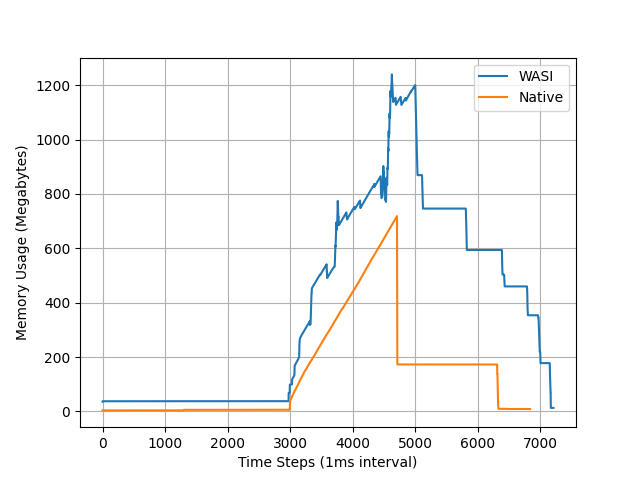
\includegraphics[width=1\textwidth]{images/mass_storage_comparison.png}
  \caption{Memory usage when traversing the file tree and reading the file contents. At the end of reading the largest file (678MB), the \acrshort{WASI} program will consume 72.5\% more memory than the native counterpart.}
  \label{fig:mass_storage_memory_comparison}
\end{figure}



\subsection{Traversing file tree from mass storage device}
\label{section:travering_file_tree_memory}
A less memory-intensive benchmark was also performed to check how \acrshort{WASI} memory usage would compare when using less memory. This benchmark uses the same test methodology as Section \ref{section:reading_files_memory}, except that it will not read out the file contents. The file tree has also changed and now contains 11947 files, with a total size of 3.25GB.

\subsubsection{Results}

Figure \ref{fig:mass_storage_file_tree_comparison} shows the results of the benchmark. The graph contains the results of the total memory usage of both programs, and also contains the \acrshort{WASI} results without the initial memory occupied by Wasmtime. This is a useful metric, as a program utilizing the \acrshort{USB} \acrshort{API} can be part of a larger piece of code, where the initial memory overhead of Wasmtime gets \textit{distributed} between all components and can be neglected.

The first 3000 measurements show the memory usage from when the program is sleeping for three seconds, as described in Section \ref{section:reading_files_memory_test_setup}. The memory of both native and \acrshort{WASI} programs are similar, not accounting for the initial Wasmtime memory usage. Furthermore, the \acrshort{WASI} memory usage is slightly better at the start, but this is likely caused by applying the correction. Once the useful program code starts, memory spikes for both programs. However, the \acrshort{WASI} (corrected) program consumes approx. 63MB of memory, 69.8\% more than the native's 37.1 MB memory usage.

\begin{figure}[H]
  \centering
  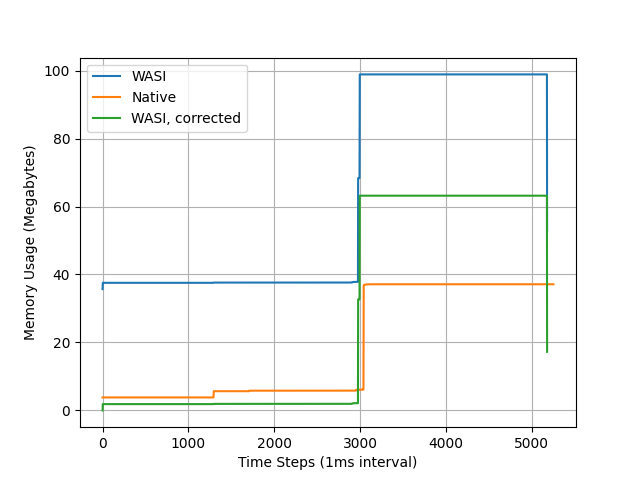
\includegraphics[width=1\textwidth]{images/mass_storage_memory_filetree_with_correction.png}
  \caption{Memory usage when traversing the file tree. The \acrshort{WASI} program consumes 69.8\% more memory than the native counterpart.}
  \label{fig:mass_storage_file_tree_comparison}
\end{figure}